\documentclass[,man,mask]{apa6}
\usepackage{lmodern}
\usepackage{amssymb,amsmath}
\usepackage{ifxetex,ifluatex}
\usepackage{fixltx2e} % provides \textsubscript
\ifnum 0\ifxetex 1\fi\ifluatex 1\fi=0 % if pdftex
  \usepackage[T1]{fontenc}
  \usepackage[utf8]{inputenc}
\else % if luatex or xelatex
  \ifxetex
    \usepackage{mathspec}
  \else
    \usepackage{fontspec}
  \fi
  \defaultfontfeatures{Ligatures=TeX,Scale=MatchLowercase}
\fi
% use upquote if available, for straight quotes in verbatim environments
\IfFileExists{upquote.sty}{\usepackage{upquote}}{}
% use microtype if available
\IfFileExists{microtype.sty}{%
\usepackage{microtype}
\UseMicrotypeSet[protrusion]{basicmath} % disable protrusion for tt fonts
}{}
\usepackage{hyperref}
\hypersetup{unicode=true,
            pdftitle={Beyond p-values: Utilizing Multiple Methods to Evaluate Evidence},
            pdfauthor={K. D. Valentine, Erin M. Buchanan, John E. Scofield, \& Marshall T. Beauchamp},
            pdfkeywords={null hypothesis testing, p-values, Bayes Factors, Observation Oriented
Modeling, evidence},
            pdfborder={0 0 0},
            breaklinks=true}
\urlstyle{same}  % don't use monospace font for urls
\usepackage{graphicx,grffile}
\makeatletter
\def\maxwidth{\ifdim\Gin@nat@width>\linewidth\linewidth\else\Gin@nat@width\fi}
\def\maxheight{\ifdim\Gin@nat@height>\textheight\textheight\else\Gin@nat@height\fi}
\makeatother
% Scale images if necessary, so that they will not overflow the page
% margins by default, and it is still possible to overwrite the defaults
% using explicit options in \includegraphics[width, height, ...]{}
\setkeys{Gin}{width=\maxwidth,height=\maxheight,keepaspectratio}
\IfFileExists{parskip.sty}{%
\usepackage{parskip}
}{% else
\setlength{\parindent}{0pt}
\setlength{\parskip}{6pt plus 2pt minus 1pt}
}
\setlength{\emergencystretch}{3em}  % prevent overfull lines
\providecommand{\tightlist}{%
  \setlength{\itemsep}{0pt}\setlength{\parskip}{0pt}}
\setcounter{secnumdepth}{0}
% Redefines (sub)paragraphs to behave more like sections
\ifx\paragraph\undefined\else
\let\oldparagraph\paragraph
\renewcommand{\paragraph}[1]{\oldparagraph{#1}\mbox{}}
\fi
\ifx\subparagraph\undefined\else
\let\oldsubparagraph\subparagraph
\renewcommand{\subparagraph}[1]{\oldsubparagraph{#1}\mbox{}}
\fi

%%% Use protect on footnotes to avoid problems with footnotes in titles
\let\rmarkdownfootnote\footnote%
\def\footnote{\protect\rmarkdownfootnote}


  \title{Beyond \emph{p}-values: Utilizing Multiple Methods to Evaluate Evidence}
    \author{K. D. Valentine\textsuperscript{1}, Erin M. Buchanan\textsuperscript{2},
John E. Scofield\textsuperscript{1}, \& Marshall T.
Beauchamp\textsuperscript{3}}
    \date{}
  
\shorttitle{Multiple Methods}
\affiliation{
\vspace{0.5cm}
\textsuperscript{1} University of Missouri\\\textsuperscript{2} Missouri State University\\\textsuperscript{3} University of Missouri - Kansas City}
\keywords{null hypothesis testing, p-values, Bayes Factors, Observation Oriented Modeling, evidence}
\usepackage{csquotes}
\usepackage{upgreek}
\captionsetup{font=singlespacing,justification=justified}

\usepackage{longtable}
\usepackage{lscape}
\usepackage{multirow}
\usepackage{tabularx}
\usepackage[flushleft]{threeparttable}
\usepackage{threeparttablex}

\newenvironment{lltable}{\begin{landscape}\begin{center}\begin{ThreePartTable}}{\end{ThreePartTable}\end{center}\end{landscape}}

\makeatletter
\newcommand\LastLTentrywidth{1em}
\newlength\longtablewidth
\setlength{\longtablewidth}{1in}
\newcommand{\getlongtablewidth}{\begingroup \ifcsname LT@\roman{LT@tables}\endcsname \global\longtablewidth=0pt \renewcommand{\LT@entry}[2]{\global\advance\longtablewidth by ##2\relax\gdef\LastLTentrywidth{##2}}\@nameuse{LT@\roman{LT@tables}} \fi \endgroup}


\DeclareDelayedFloatFlavor{ThreePartTable}{table}
\DeclareDelayedFloatFlavor{lltable}{table}
\DeclareDelayedFloatFlavor*{longtable}{table}
\makeatletter
\renewcommand{\efloat@iwrite}[1]{\immediate\expandafter\protected@write\csname efloat@post#1\endcsname{}}
\makeatother
\usepackage{lineno}

\linenumbers

\authornote{

Correspondence concerning this article should be addressed to K. D.
Valentine, 210 McAlester Ave, Columbia, MO 65211. E-mail:
\href{mailto:Katy.valentine3@gmail.com}{\nolinkurl{Katy.valentine3@gmail.com}}.
On behalf of all authors, the corresponding author states that there is
no conflict of interest.}

\abstract{
Null hypothesis significance testing (NSHT) is cited as a threat to
validity and reproducibility. While many individuals suggest we focus on
altering the \emph{p}-value at which we deem an effect significant, we
believe this suggestion is short-sighted. Alternative procedures (i.e.,
Bayesian analyses and Observation Oriented Modeling; OOM) can be more
powerful and meaningful to our discipline. However, these methodologies
are less frequently utilized and are rarely discussed in combination
with NHST. Herein, we discuss three methodologies (NHST, Bayesian Model
comparison, and OOM), then compare the possible interpretations of three
analyses (ANOVA, Bayes Factor, and an Ordinal Pattern Analysis) in
various data environments using a frequentist simulation study. We find
that changing significance thresholds has little effect on conclusions.
We find that evaluating multiple estimates as evidence of an effect
allows for more robust and nuanced reports of findings. These findings
suggest the need to redefine evidentiary value and reporting practices.


}

\usepackage{amsthm}
\newtheorem{theorem}{Theorem}[section]
\newtheorem{lemma}{Lemma}[section]
\theoremstyle{definition}
\newtheorem{definition}{Definition}[section]
\newtheorem{corollary}{Corollary}[section]
\newtheorem{proposition}{Proposition}[section]
\theoremstyle{definition}
\newtheorem{example}{Example}[section]
\theoremstyle{definition}
\newtheorem{exercise}{Exercise}[section]
\theoremstyle{remark}
\newtheorem*{remark}{Remark}
\newtheorem*{solution}{Solution}
\begin{document}
\maketitle

Recent events in psychological science have prompted concerns within the
discipline regarding research practices and ultimately the validity and
reproducibility of published reports (Etz \& Vandekerckhove, 2016;
Lindsay, 2015; Open Science Collaboration, 2015; van Elk et al., 2015).
One often discussed matter is over-reliance, abuse, and potential
hacking of \emph{p}-values produced by frequentist null hypothesis
significance testing (NHST), as well as misinterpretations of NHST
results (Gigerenzer, 2004; Ioannidis, 2005; Simmons, Nelson, \&
Simonsohn, 2011). We agree with these concerns and believe that many
before us have voiced sound, generally accepted opinions on potential
remedies, such as an increased focus on effect sizes (Cumming, 2008;
Lakens, 2013; Maxwell, Lau, \& Howard, 2015; Nosek, Spies, \& Motyl,
2012). However, other suggestions have been met with less enthusiasm,
including a recent article by Benjamin et al. (2018) advocating that
researchers should begin thinking only of \emph{p}-values less than .005
as \enquote{statistically significant}, thus changing \(\alpha\) levels
to control Type I error rates. Additionally, Pericchi and Pereira (2016)
promote the use of fluctuating \(\alpha\) levels as a function of sample
size to assist with these errors. We argue it is not the threshold, or
critical \emph{p}, that needs to be rethought when seeking evidence, but
rather if a \emph{p}-value should be utilized at all, and, if so, what
that \emph{p}-value can tell you in relation to other indicators. While
NHST and \emph{p}-values may have merit, researchers have a wealth of
other statistical tools available to them. We believe that improvements
may be made to the sciences as a whole when individuals become aware of
the tools available to them and how these methods may be used, either
alone or in combination, to strengthen understanding and conclusions.
These sentiments have been shared by the American Statistical
Association who recently held a conference focusing on going beyond
NHST, expanding their previous stance \emph{p}-values (Wasserstein \&
Lazar, 2016).

Therefore, we undertook this project to show researchers how two
alternative paradigms compare to NHST in terms of their methodological
design, statistical interpretations, and comparative robustness. Herein,
we will discuss the following methodologies: NHST, Bayes Factor
comparisons, and Observation Oriented Modeling. The three approaches
will be compared via this simulated data using a three timepoint
repeated measures design with a Likert-type scale as the outcome
variable. One goal of this study is to introduce social scientists to
Observation Oriented Modeling (OOM), as it is a relatively new paradigm
that is readily interpretable and, as we will show, useful in these
contexts. Additionally, we aim to discuss the conclusions these three
methods would make given the same data, and to compare how often these
methodologies agree within different data environments (i.e., given
varying sample sizes and effect sizes). We hope that by discussing these
methodologies in terms of a simple statistical analysis researchers will
be able to easily compare and contrast methodologies. For this
discussion, it is important to understand their historical background,
procedural steps, and limitations, which are outlined below. After this
discussion, we describe a simulation study comparing methodologies and
\(\alpha\) criteria, and end with potential implications for
researchers.

\hypertarget{null-hypothesis-significance-testing}{%
\section{Null Hypothesis Significance
Testing}\label{null-hypothesis-significance-testing}}

\hypertarget{history}{%
\subsection{History}\label{history}}

Many attribute the frequentist NHST procedure to Ronald A. Fisher
(Fisher, 1932). However, Fisher's ideas are a far cry from the NHST
procedure implemented today. Fisher believed in creating one
\enquote{null} hypothesis, which he described as a hypothesis to be
\enquote{nullified}, or shown incorrect, not as a zero-difference
hypothesis (Lehmann, 2011). He also believed that the use of any omnibus
level of significance showed a \enquote{lack of statistical thinking}
(Gigerenzer et al., 2004). He instead believed we should report the
exact significance value of a test and let others make their own
decision about the claims, which is more in line with the typical
reporting recommendations provided by the American Psychological
Association (American Psychological Association, 2010). Fisher spoke of
this work to William Gosset, the man who created the Student's
\emph{t}-test and contributed work on the correlation coefficient
(Lehmann, 2011). Gosset in turn discussed the idea of an alternative
hypothesis, a piece not included in Fisher's procedure, with decision
theorist Egon Pearson.

From this discussion, Egon Pearson and Jerzy Neyman created
Neyman-Pearson decision theory. This theory consists of two hypotheses
(i.e., null and alternative) and a binary decision criteria (i.e.,
significant or not, Lehmann, 1993). However, this procedure created the
possibility of researcher decision errors (Dienes, 2008). A researcher
may falsely reject the null hypothesis (Type I error, \(\alpha\)) or
falsely fail to reject the null (Type II error, \(\beta\)). \(\alpha\)
levels set the binary decision criteria, which are used as the critical
\emph{p}-value for hypothesis testing (i.e., \emph{p} \textless{} .05),
and are thus seen as evidence to reject the null hypothesis. \(\beta\)
and power are inherently linked (Power = 1-\(\beta\)), so as the
likelihood of finding a true effect increases beta decreases (Maxwell \&
Delaney, 2004). Although \(\alpha\) values can be chosen to be quite
small, and methods (such as decreasing error variance or using a
one-tailed test in contrast to a two-tailed test) can decrease \(\beta\)
values as well, a researcher can never know if they have made the
correct decision, or a decision error. Thus, Neyman and Pearson clearly
state that a hypothesis should not be blindly supported based solely on
the estimates of one statistical test, and that replication and
reproduction of results are imperative. The recent work of the Open
Science Collaboration (2015) has also highlighted the need for
replication studies and interpretation of results in an appropriate
context. Additionally, Neyman and Pearson emphasized that use of set
\(\alpha\)s and \(\beta\)s is illogical and sought instead for
researchers to adjust their analysis to the needs of the particular task
at hand (Gigerenzer, 2004).

\hypertarget{typical-nhst-procedure}{%
\subsection{Typical NHST Procedure}\label{typical-nhst-procedure}}

Neither Fisher's hypothesis testing, nor Neyman-Pearson decision theory
quite match the NSHT procedure as it is taught and applied today.
Psychologists have largely adopted an amalgamation of the two
approaches. Here, we attempt to outline what we believe is the most
appropriate way to carry out the traditional NHST procedure in the
context of a repeated measures ANOVA with three levels, although we note
that this set of steps is not necessarily how researchers carry out the
procedure in practice:

\begin{enumerate}
\def\labelenumi{\arabic{enumi})}
\tightlist
\item
  Create two hypotheses, one to be \enquote{nullified} and one
  \enquote{alternative} hypothesis. Within this repeated measures
  framework, most researchers would define a null hypothesis (\(H_0\))
  that indicates of all three time point population means are equal. The
  alternative hypothesis (\(H_A\)) would then be that not all of the
  population means are equal. These can be operationalized in our
  example data as follows (note that for \(H_A\), we use a common short
  hand to denote the model wherein any difference is hypothesized across
  the possible combinations of {[}in{]}equality):
\end{enumerate}

\[
\begin{aligned}
  H_0: \mu_1 = \mu_2 = \mu_3 \\
  H_A: \mu_1 \neq \mu_2 \neq \mu_3
\end{aligned}
\]

\begin{enumerate}
\def\labelenumi{\arabic{enumi})}
\setcounter{enumi}{1}
\item
  Select an \(\alpha\) level that is appropriate given the context of
  your research, your analysis plan, and your research question, and do
  not blindly adopt an omnibus critical \emph{p}-value (Lakens et al.,
  2018; Lehmann, 2011). Again, we reiterate that \(\alpha\)
  justification and selection is not necessarily how all researchers
  approach these tests.
\item
  Compute your given analysis and identify the corresponding
  \emph{p}-value. If your \emph{p}-value is less than the chosen
  \(\alpha\), reject the null hypothesis and state that there appear to
  be differences between some of your population means; however, if your
  \emph{p}-value is greater than or equal to the value selected, do not
  reject the null hypothesis, and state that a difference between the
  population means could not be supported.
\end{enumerate}

While the NHST procedure itself gives us testable models, the specific
analysis used to test these models here, the repeated measures ANOVA
with three levels, requires some additional assumptions that must be met
before an analysis is begun (Tabachnick \& Fidell, 2012). Data need to
have no outlying or influential observations. Data must have a normal
sampling distribution, be linearly related, and have independent errors.
Depending on the statistical test, data must also be checked for equal
variances, sphericity, and additivity. These assumptions can be checked
and, if necessary, corrected for; however, violations of these
assumptions can lead to inaccurate decisions and attenuated power.
Further, with many analysis programs, data are required to have no
missing values.

While this approach is widely used, there are many limitations
associated with it. First, this method can be sensitive to violations of
the stated assumptions, and especially, if the sample size is not large
enough to create a normal sampling distribution (Tabachnick \& Fidell,
2012). Even if assumptions are met, or nonparametric tests are
implemented (e.g., for situations where a normal distribution assumption
cannot be met), this methodology does not allow a researcher to state
anything about the absence of an effect (i.e., no true differences).
Through traditional NHST, one can only discuss evidence regarding the
alternative hypothesis; one can never support the null hypothesis
through this procedure. Given the recent findings regarding
reproducibility, showing support for the absence of an effect can be
even more crucial than showing support for the presence of an effect
(Bakker, van Dijk, \& Wicherts, 2012; Lakens, 2017).

\hypertarget{bayes-factors}{%
\section{Bayes Factors}\label{bayes-factors}}

\hypertarget{history-1}{%
\subsection{History}\label{history-1}}

Thomas Bayes was a statistician and Presbyterian minister whose works
are still influential today (Bellhouse, 2004). Bayes' theorem solved the
inverse probability problem, namely that through the frequentist
approach, one can only know the probability of data existing given a
hypothesis being true, never the probability of a hypothesis being true
given that the data exist (Dienes, 2008). Bayes' theorem allows one to
calculate the probability of a hypothesis given some data (posterior
belief) by using how probable one believes the hypothesis to be before
data was collected (prior belief) and how probable one believes the data
to be given one's hypothesis (likelihood). Thus, with his theorem,
researchers are able to update (through the use of the likelihood) our
initial beliefs (our prior) given some data (Gelman, Carlin, Stern, \&
Rubin, 2013). Pierre-Simon Laplace pioneered Bayesianism and advocated
for a broader interpretation of this theorem (De Laplace, 1774). The use
of Bayesian statistics has been suggested as an NHST alternative
(Dienes, 2014; Wagenmakers, 2007), but this approach has largely been
undervalued in favor of frequentist methods as, until recently, Bayesian
analysis required considerable computational effort. However, today we
possess the technology necessary to efficiently conduct Bayesian
analyses. While open source software, such as \emph{R} and JASP, require
minimal learning to be able to effectively operate (Morey \& Rouder,
2015), researchers will need to invest more effort to understand the
focus and interpretation of Bayes Factor (BF) comparisons as they differ
from traditional NHST.

The Bayesian framework can be viewed as a continuum, with objective
Bayesian analyses on one end, and subjective Bayesian analyses on the
other (Press, 2002). While this topic could lend itself to its own
manuscript, here we will simply summarize the two endpoints, and discuss
where our analysis may be perceived to fall on the line. Objective
Bayesian analysis is closest to frequentist theory, as the aim is to
minimize the influence of priors through the use of non-informative
priors (such as Jefferys priors that are designed to be invariant under
reparameterization Datta \& Ghosh, 1996); thus, the data are allowed to
maximally effect the posterior distribution. Further, objective Bayesian
methods are influenced by the same quality criteria that frequentist
methods used, including Type I error rate and power (Sellke, Bayarri, \&
Berger, 2001). On the other end, subjective Bayes analyses include
rigorously informed priors so that current knowledge can play a large
role in the posterior. Our current analysis splits these two; we do not
utilize completely uniformed (objective) priors, as we can adjust for
basic knowledge of the constraints of our data type. Given the usual
lack of information about underlying distributions, a wider band of
inclusion was used for prior information. The \emph{BayesFactor} package
(Morey \& Rouder, 2015) assists greatly in the choice of prior and is
especially user-friendly for applied researchers, as it makes use of
recommended default priors that have been chosen to be safe to assume
under a broad range of data and topics (Rouder, Morey, Speckman, \&
Province, 2012; Rouder, Speckman, Sun, Morey, \& Iverson, 2009). Instead
of conventional \emph{F}, \emph{t}, and \emph{p}-values, a ratio of the
likelihood of the alternative model to the null is report, usually
\(BF_{10}\). For instance, \(BF_{10}\) = 20 would indicate that the
effects model is favored 20 to 1 over the null model. Conversely, if the
\(BF_{10}\) were 0.10, the null model is favored 10 to 1 over the
effects model.

\hypertarget{typical-procedure}{%
\subsection{Typical Procedure}\label{typical-procedure}}

The procedure behind BF comparisons requires two steps.

\begin{enumerate}
\def\labelenumi{\arabic{enumi})}
\tightlist
\item
  One must design two models for the data. For our purposes, the first
  of these models will be the null model, which states that there are no
  differences between means (\(\mu\); i.e., all of our observed values
  \(X_{i}\), regardless of which time point they were assessed at
  \(X_{ij}\), arise from a normal distribution \emph{N} with some mean
  \(\mu\) and variance \(\sigma^2\)). The second model for these
  analyses is the effects model, which states that each mean (\(\mu\))
  is allowed to be different from the grand mean by some amount
  (\(\delta\); as we now have observations being drawn from three
  potential normal distributions, all of which may have a different mean
  value, but the same variance). These can be operationalized as
  follows:
\end{enumerate}

\[
\begin{aligned}
  H_0: X_{ij} \sim N(\mu, \sigma^2) \\
  H_A: X_{ij} \sim N(\mu + \delta_i, \sigma^2)
\end{aligned}
\] In designing these models, one must choose the prior distributions
that are believed to describe the data. Reasonable expectancies of where
the data lie should be incorporated in this decision based on previous
research into the studied phenomena (Rouder et al., 2012).

\begin{enumerate}
\def\labelenumi{\arabic{enumi})}
\setcounter{enumi}{1}
\tightlist
\item
  Analyze the data given the selected priors and models. Consider the BF
  and use the \(BF_{10}\) as evidence of how one should update their
  beliefs about the models.
\end{enumerate}

Based on the flexibility of the analysis, the only assumption that needs
to be made is that data exists such that two competing, plausible models
with different constraints may be specified.

Bayesian inference improves upon the traditional frequentist point of
view by allowing not only a clear interpretation of the evidence
provided by the data, but also the ability to speak in favor of the null
hypothesis. It is important to note that while previous work has
indicated that \emph{p}-values and BF largely agree on which hypothesis
should be supported, they differ in the strength of that conclusion,
especially when \emph{p}-values were slightly lower than \(\alpha\)
(i.e., .05 to .01; Wetzels et al., 2011). However, some limitations do
arise in this paradigm. Bayesian analyses require the researcher to take
an active role in the choice of prior distributions for the phenomenon
they are modeling, and this decision can take some effort to fully
understand; however, in the meantime, there are packages such as
\emph{BayesFactor} that provide the researcher simple default options
that can readily lend themselves to many research areas with little fear
of being outrageous specifications. Further, unlike NHST, Bayesian
analyses do not necessarily control long-run error rates, as the focus
is on updating current model beliefs. Another concern that many
researchers have is that these analyses are necessarily sensitive to
prior choice. However, research has shown that the choice of priors has
essentially no effect on conclusions when sufficient data has been
collected as the priors give way to the weight of the data (Klugkist \&
Hoijtink, 2007; Rouder et al., 2012) and when reasonable priors are
considered, data are only mildly sensitive to these (Haaf \& Rouder,
2017). Finally, many believe Bayesian analysis to be too computationally
intensive to complete. However, many simple programs, packages, and
tutorials exist to help ease the transition from frequentist to Bayesian
analysis (JASP Team, 2017; Kruschke, 2014; Morey \& Rouder, 2015).

\hypertarget{observation-oriented-modeling}{%
\section{Observation Oriented
Modeling}\label{observation-oriented-modeling}}

\hypertarget{history-2}{%
\subsection{History}\label{history-2}}

James Grice argues that our problems as a science go beyond use of NHST
and extend into the philosophical ideas underpinning our research.
Therefore, he developed a new paradigm called Observation Oriented
Modeling (OOM, Grice, 2011, 2014; Grice, Barrett, Schlimgen, \&
Abramson, 2012). He reasons that by viewing psychology through the lens
of philosophical realism, instead of positivism, we should be able to
properly and effectively conduct research and analyze data. In contrast
to positivism (i.e., which is solely concerned with finding an effect,
not with how the effect occurred), philosophical realism holds that the
causal structure of nature can be understood through scientific
investigation. The goal is then to understand the causal mechanisms that
give rise to the patterns observed in a given set of observations, which
in here would refer to data. Switching to this philosophy allows for
techniques that match the daily activities of social scientists in their
endeavors to unravel the story of how humans operate. Using OOM, a
researcher does not focus on population parameters and the various
assumptions underlying statistical tests (e.g., random sampling,
normality, homogeneity of population treatment differences, etc.).

Generally speaking, this approach can handle any type of data, including
ordinal rankings and frequency counts, as all analyses are calculated in
the same general fashion (see Valentine \& Buchanan, 2013 for an
example). This simplicity occurs because OOM works on the deep structure
of the data. Through observational definition, the program separates
these units into binary code. Deep structures can be arranged to form a
matrix, which can then be manipulated via matrix algebra, binary
Procrustes rotation, and other operations to investigate the data. The
most important values from any OOM analysis are the PCC (percent correct
classification) values. These values represent the summation of how well
an individual's responses matched the stated or expected pattern or, in
the case of causal modeling, how many of the individual's conformed to a
given cause. Complete matches are the proportion of observations that
match the researcher-designated pattern on all dimensions. For example,
in a three-level Ordinal Pattern Analysis (OPA), a person would be
tallied as a \enquote{complete match} if the ordinal pattern of his/her
data matched the expected ordinal pattern across all three levels.
Imagine we have set a pattern that designates Time 1 \textless{} Time 2
\textless{} Time 3. For example, imagine we have data for two
hypothetical individuals. Person A has values of 3, 4, and 5 at
timepoints 1, 2, and 3, respectively, while person B has values of 4, 5,
and 2. We can see that Person A matched the pattern completely, and
therefore would be counted in the PCC value. However, while person B
matched the first part of our pattern (time 1 less than time 2), they
did not match on the third point of our pattern (time 2 less than time
3); thus, they would not be counted in the PCC value. As the PCC is
simply the percentage of individuals in a sample whose responses match
the expected ordinal pattern perfectly, its computation is therefore not
based on means or variances, but on the basis of the observations
themselves. The PCC value replaces all of the conventional values for
effect size used in statistical analyses.

The analysis we focus on here (OPA) does not form any type of linear or
nonlinear equation or regression, but simply looks for those individuals
who match the expected ordinal pattern (Grice, Craig, \& Abramson,
2015). The main point of the analysis, then, is to see how many people
fit the expected pattern which is based on a causal theory. If all
causes are accounted for in the study and observations have been made
with sufficient precision and accuracy, then 100\% of the persons should
fit the expected pattern; otherwise, a lower PCC value will be expected
and it is up to the researcher to determine how high a PCC must be in
order to support an inference to the causal mechanism.

In OOM, traditional \emph{p}-values are no longer utilized (Grice,
2011). As a secondary form of reference value, a chance value
(\emph{c}-value) is obtained, which is a type of randomization test in
which the researcher determines the number of randomized trials for the
test (e.g.~1,000 or 5,000 randomized versions of actual observations).
This procedure is akin to permutation tests, where PCCs are computed for
the randomized data to form a distribution. The observed PCC is then
compared to these values, and the c-value (which is an empirical
probability) is determined. If the randomized data sets fit the pattern
as well as or better than the actual data does, the \emph{c}-value will
be high (close to 1). Low \emph{c}-values (close to 0) indicate a
pattern of observations that is improbable (i.e., unlikely produced by
chance) when compared to randomized versions of the same data. Although
low \emph{c}-values, like low \emph{p}-values, are desirable,
\emph{c}-values do not adhere to a strict cut-off and should be
considered a secondary form of confirmation for the researcher that
their results are distinct.

\hypertarget{typical-procedure-1}{%
\subsection{Typical Procedure}\label{typical-procedure-1}}

OPA is analogous to repeated measures ANOVA and contains two steps.

\begin{enumerate}
\def\labelenumi{\arabic{enumi})}
\tightlist
\item
  Designate the expected ranked pattern: each variable as being higher,
  lower, or equal to the other variables. For instance, for our analyses
  we defined the following pattern of individual responses \(X_i\),
  whereby the first time point should be less than the second time point
  which should be less than the third time point. This pattern can be
  operationalized as follows:
\end{enumerate}

\[
  X_{i_1} < X_{i_2} < X_{i_3}   
\]

\begin{enumerate}
\def\labelenumi{\arabic{enumi})}
\setcounter{enumi}{1}
\tightlist
\item
  Analyze the data using OPA. Consider the PCC (the percentage of
  individuals matching the ordinal hypothesis) and \emph{c}-values in
  light of the data and use your best judgment as to whether or not the
  data conform to the expected pattern. This analysis only requires the
  assumption that the data exists such that a pattern may be designed.
\end{enumerate}

As with all of these methodologies, limitations do exist. This approach
is largely concerned with patterns of responses, not with magnitudes of
differences, which may be an integral piece of information to some
researchers. Unlike all approaches mentioned before, we do not discuss
the probability of some data given our hypothesis here, and instead
focus on the observed responses of the individual and how it may or may
not behave as expected. Finally, similar to the Bayesian analysis,
long-run error rates are not discussed in this methodology.

\hypertarget{a-simulation-study}{%
\section{A Simulation Study}\label{a-simulation-study}}

\hypertarget{simulated-data}{%
\subsection{Simulated Data}\label{simulated-data}}

In this study, we generated 20,000 datasets by manipulating sample size
and effect size for a repeated measures design with three levels. A
repeated measures design was chosen as it is widely used across many
disciplines of psychology. These datasets were created using the
\emph{mvtnorm} package in \emph{R} (Genz et al., 2017), and all code for
simulations can be found at
\url{https://osf.io/u9hf4/?view_only=1caa9092868b4d7aadb9a83a31a979cd}.
Interested readers can easily adapt the \emph{R} code to incorporate
different research designs. Likert data, ranging from 1 to 7, was
created by rounding \emph{mvtnorm} estimates to whole numbers and
truncating any data points out side of the appropriate range (i.e.,
values \textless{} 1 were rounded to 1, and values \textgreater{} 7 were
rounded to 7). We specifically chose Likert-type data as this data type
is one of the most common data types utilized by most social scientists.
Additionally, we add to the literature as other simulations have chosen
to use completely continuous data (i.e., simulated numbers are often
precise to 10+ decimals, which is unlikely for traditional sampling).
The simulated data did increase in skew with this procedure from
approximately no skew (i.e., \textless{}0.01) to approximately 0.40 for
the smallest and no effect conditions; however, these values closely
resembled a normal distribution with the use of \emph{mvtnorm}. The
population means for each level were set to 2.5, 3.0, and 3.5, and
pairwise effect sizes (e.g., the comparison between time 1 v. time 2 and
time 2 v. time 3) were manipulated by adjusting the standard deviation
to create negligible effects (\emph{SD} = 3.39, \emph{d} = 0.10), small
effects (\emph{SD} = 3.00, \emph{d} = 0.20), medium effects (\emph{SD} =
0.50, \emph{d} = 0.50), and large effects (\emph{SD} = 0.10, \emph{d} =
0.80) using Cohen (1992)'s traditional guidelines for \emph{d}
interpretation. The smallest effect size was set such that Likert style
data could still be retained with the smallest possible effect size.
Sample size was manipulated at 10, 30, 100, 500, and 1,000 data points.
All combinations of the five sample sizes and four effect sizes were
created, and each dataset was simulated 1,000 times, totaling 20,000
datasets.

The advantage of using \emph{mvtnorm} and set \emph{SDs} for each group
was the ability to approximate the assumptions of normality by randomly
generating from a multivariate normal distribution, and homogeneity by
setting equal \emph{SDs} for each group. In a repeated measures design,
the assumption of sphericity was met by setting the correlations between
levels in \emph{mvtnorm} to zero. By maintaining the lowest level of
relationship between levels, we additionally controlled for power and
examined situations of significance given the lowest power scenario.
During the data simulation, the standard deviation of the difference
scores was examined to maintain differences greater than zero,
especially for low \emph{N} simulations.

\hypertarget{analyses-performed}{%
\subsection{Analyses Performed}\label{analyses-performed}}

\hypertarget{descriptive-statistics}{%
\subsubsection{Descriptive Statistics}\label{descriptive-statistics}}

Means, mean differences between levels, and the confidence intervals for
each mean can be found in the complete dataset online,
\url{https://osf.io/u9hf4/?view_only=1caa9092868b4d7aadb9a83a31a979cd}.
For each simulation, we also calculated \emph{d} values using the
standard deviation of the difference score as the denominator
(\(d_{z}\), Lakens, 2013). The \emph{MOTE} library was used to calculate
the non-central confidence interval for each \emph{d} value as well
(Buchanan, Valentine, \& Scofield, 2017; Cumming, 2014). This data was
mainly used to determine if simulations were meeting expected values
overall.

\hypertarget{parametric-nhst---repeated-measures-anova}{%
\subsubsection{Parametric NHST - Repeated Measures
ANOVA}\label{parametric-nhst---repeated-measures-anova}}

Repeated measures ANOVA using the \emph{ezANOVA()} function in the
\emph{ez} library was utilized with type three sum of squares (Lawrence,
2017). This style of ANOVA is used to compare the same individuals
across multiple or all conditions in an experiment. The null hypothesis
states that there are no significant differences between population
means, and the research hypothesis posits that there are differences
between some population means, but does not specify which population
means may differ, just that one or more will differ as the alternative.
This test uses the \emph{F} distribution focusing on \emph{p} values.

To determine where differences may exist, \emph{post hoc} dependent
\emph{t}-tests are normally analyzed in the event of a significant
\emph{F}-ratio. We did not run all pairwise comparisons, instead
focusing on the linear trend simulated by comparing level one to two and
level two to three. This set of comparisons also controlled the effect
size between comparisons, as comparing level one to three would have
doubled the effect size. However, we assumed that typical researchers
might compare all three pairwise combinations in practice and used a
Bonferroni correction across all three possible pairwise combinations to
calculate \emph{p} values for \emph{post hoc} tests. Therefore, while we
only discuss the two comparisons, we utilized the more stringent cutoff
of the Bonferroni correction as we believe this procedure would be how
the majority of researchers would handle the data. Interested readers
can find all three comparison values in the complete dataset online.
Following traditional usage, a \emph{p}-value of less than .05 was
binned as significant, whereas \emph{p}-values ranging from .10 to .05
were binned as marginally significant. Any \emph{p}-values larger than
.10 were binned as non-significant. A second set of \emph{p}-value
comparisons was calculated given Benjamin et al. (2018)'s suggestion to
change \(\alpha\) criterion to less than .005. Any \emph{p}-value less
than .005 was binned as significant, while data ranging from .005 to .10
was marginal or suggestive, and \emph{p} \textgreater{} .10 was
non-significant.

\hypertarget{bayesian-analysis-bayes-factor}{%
\subsubsection{Bayesian Analysis: Bayes
Factor}\label{bayesian-analysis-bayes-factor}}

We compared a null model with one grand mean for all three levels to an
effects model wherein means were allowed to differ using the
\emph{BayesFactor} package (Morey \& Rouder, 2015). The default in this
package is a Jeffreys prior with a fixed rscale (0.5) and random rscale
(1.0). BF were calculated, and follow up \emph{t}-test BFs were computed
for the same two comparisons as in the previous models using default
priors from the \emph{BayesFactor} package (e.g., Jeffreys prior for
population variance, Cauchy prior for standardized effect size). To
compare Bayesian results to other statistical methods, we used
recommendations from Kass and Raftery (1995) to bin results into weak
evidence (BFs \textless{} 3), positive evidence (e.g., akin to marginal
\emph{p}-values, BFs = 3-20), and strong evidence (BFs \textgreater{}
20). We must stress here that BF interpretation should focus on
understanding the odds of model ratios, not necessarily the presence or
absence of an effect. However, given that we wanted to compare the
conclusions one would reach given this data in a Bayesian paradigm to
that of a frequentist paradigm, these bins are used as a convenient
comparison to the frequentist procedures using set criteria for
interpretation (Morey, 2015). Should any reader become curious how a
different set of binning values affect our analyses, all code and data
are at their disposal at
\url{https://osf.io/u9hf4/?view_only=1caa9092868b4d7aadb9a83a31a979cd},
and this manuscript was written with the \emph{papaja} package allowing
one to view the code inline with this text (Aust \& Barth, 2017).

\hypertarget{oom-ordinal-pattern-analysis}{%
\subsubsection{OOM: Ordinal Pattern
Analysis}\label{oom-ordinal-pattern-analysis}}

An \emph{R} script of the Ordinal Pattern Analysis from Grice et al.
(2015)'s OOM program was provided from Sauer and Luebke (2016). We set
the expected ranked pattern as level one less than level two less than
level three. Once this pattern was defined, we then analyzed the data to
see if each individual's set of observations matched this expected
ordinal pattern. PCC values were generated, and \emph{c}-values were
computed by randomizing the data 1,000 times. Solely for purposes of
comparison, we used the following significance coding schema:
significant studies had a high PCC value (.50 \textless{} PCC
\textless{} 1.00) and a low \emph{c}-value (\emph{c} \textless{} .05),
marginal studies had a high PCC value and a moderate \emph{c}-value (.05
\textless{} \emph{c} \textless{} .10), and non-significant studies had
low PCC values (PCC \textless{} .50), regardless of their
\emph{c}-values. Again, we must stress that this paradigm eschews
binning estimates and that our use of bins was a) discussed and decided
upon before data analysis, and b) created only for the purposes of
comparing this new methodologies possible conclusions to that of a
frequentist framework. We welcome interested readers to explore the data
more, defining their own bins and viewing the affects, by viewing and
editing our code online.

\hypertarget{results}{%
\section{Results}\label{results}}

\hypertarget{percent-of-estimates}{%
\subsection{Percent of Estimates}\label{percent-of-estimates}}

For all simulations, we first binned the estimates into significant,
marginal, and non-significant effect categories as described in the
Analyses Performed section above. Next, we calculated the percentage of
these analyses that would be classified into each of these categories,
separated about by statistical analysis, sample size, and effect size.
These estimates were binned across both the overall and follow up
\emph{post hoc} tests, and the combined data are presented for this
analysis. Since all three categories of binning total to 100\%, we
present only the significant and non-significant results. Significant
critical omnibus estimates are presented in Figure
\ref{fig:effects-graph-sig}. All figures discussed in this manuscript
may be viewed as interactive graphics on our OSF page through a provided
Shiny app. In Figures with sample size on the axes, we log transformed
\emph{N} to allow for visual distinction between sample sizes, as
smaller \emph{N} values were compressed when using the \emph{N} = 10 to
1000 on the axis. Both \emph{N} and log(\emph{N}) can be found in the
Shiny app, along with the ability to zoom in to specific ranges of
sample size.

For negligible effects at \(p\) \textless{} .05 (solid lines), we found
that NSHT analyses showed a predictable Type I error bias, in that they
detected significant estimates with extremely small \emph{d} values as
sample size increased. Binned BF values showed a similar pattern, but
were more conservative with less percent significant estimates. OOM
analyses were the most conservative, essentially never detecting an
estimate in the negligible effect simulations. Small effect sizes showed
the same pattern for NHST, BF, and OOM results, with the proportion of
significant estimates increasing more rapidly and asymptoting at a
smaller sample size than negligible effects. At medium effect sizes,
NHST analyses nearly always detected significant estimates, while BF and
OOM analyses would have been considered significant around 75\% of the
time. Interestingly, with large effect sizes, OOM analyses mirrored NHST
by always detecting estimates, and BF analyses were generally more
conservative except at the largest sample size. Figure
\ref{fig:effects-graph-sig}'s dashed lines indicate the results if
values were binned at \emph{p} \textless{} .005, and the differences
between these results were very subtle. Lowering \(\alpha\) reduced the
number of significant estimates at small \emph{N} values for all four
effect sizes, with more pronounced differences at negligible and small
effect sizes. However, the graphs converged to the same conclusion that
large enough sample sizes could produce significant results at
negligible and small effect sizes.

Figure \ref{fig:effects-graph-nonsig} portrays the results for
non-significant binned simulations, which were the same for both
\(\alpha\) criterion. Across all effect sizes, BF and NHST showed
similar results, where non-significant estimates were detected at lower
sample sizes for negligible and small effect size simulations. At medium
and large effect sizes, almost all estimates would have been considered
significant, therefore, detection rates for non-significant estimates
were around zero. OOM displayed a conservative set of findings, showing
nearly 100\% non-significant estimates at negligible and small effect
sizes (mirroring results from Figure \ref{fig:effects-graph-sig}). At
medium effect sizes, approximately a quarter of estimates were
non-significant, illustrating the conservative nature of OOM
interpretations.

Figure \ref{fig:effects-pcc-d} depicts the relationship between the
effect size of time 1 minus time 2 and the corresponding PCC values.
These metrics appear to represent different concepts where effect size
measures the magnitude of the difference between two data points while
PCC disregards magnitude and represents the proportion of the sample
following the given ordinal pattern across all three time points. Given
these differences, it is interesting how well these two measures
converge together. As sample size increases, estimates for both \emph{d}
and PCC become more precise (i.e., smaller range, closer to the
simulated effect size). We believe that PCC offers researchers the
ability not only to confirm that their effect size is reasonable, but
also to better understand the pattern their data are following,
especially if an observed effect size contradicts previous literature.
For example, let us assume there is previous literature that states that
a small positive effect exists, such that responses should increase from
time 1 to time 2. Under conditions of a true small effect (\emph{d}= -
0.20) and sample size of 30, our graph shows us that it is possible to
obtain a positive medium effect size (\emph{d} = 0.50; indicating the
time 1 is more extreme than time 2). Upon finding these contradicting
results, the researcher could further seek to understand the pattern
their data are following by computing the PCC value for the experiment.
The PCC value for this example would be above .50, indicating that, in
over half of respondents the values for time 1 are less than time 2 (in
turn less than time 3, as it measures the entire pattern), even though
magnitude of change suggests that time 1 is larger than time 2. This
gives the researcher a richer piece of information, which can help to
describe their results in a more nuanced fashion.

\begin{figure}
\centering
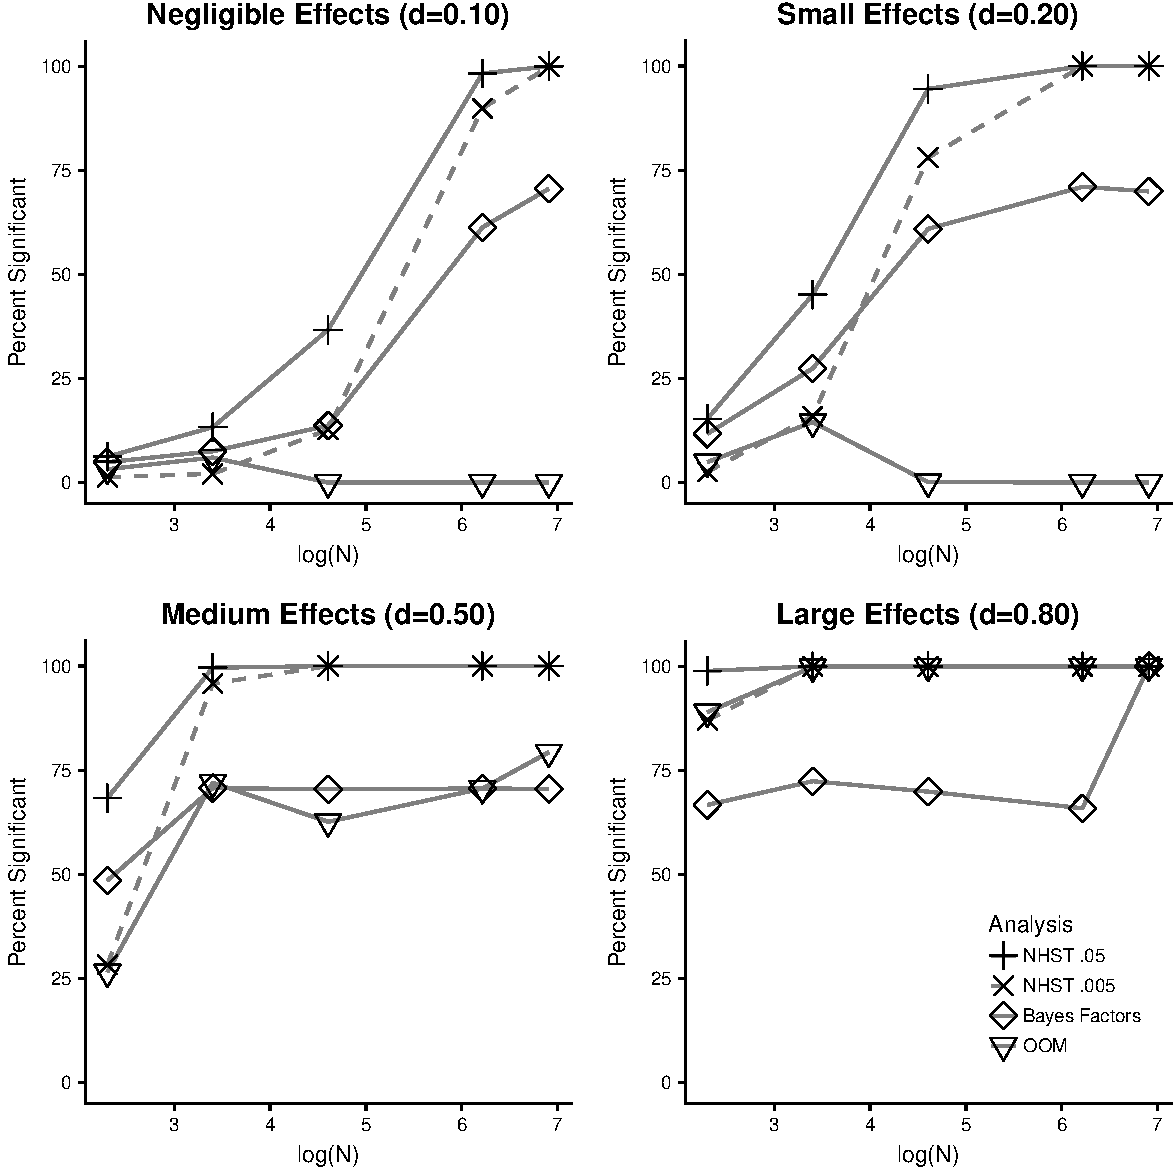
\includegraphics{alt_nhst_FINAL_files/figure-latex/effects-graph-sig-1.pdf}
\caption{\label{fig:effects-graph-sig}For NHST analyses only, percent of
significant estimates at \(p\) \textless{} .05 (solid) and \(p\)
\textless{} .005 (dashed) for each analysis given effect size and sample
size.}
\end{figure}

\begin{figure}
\centering
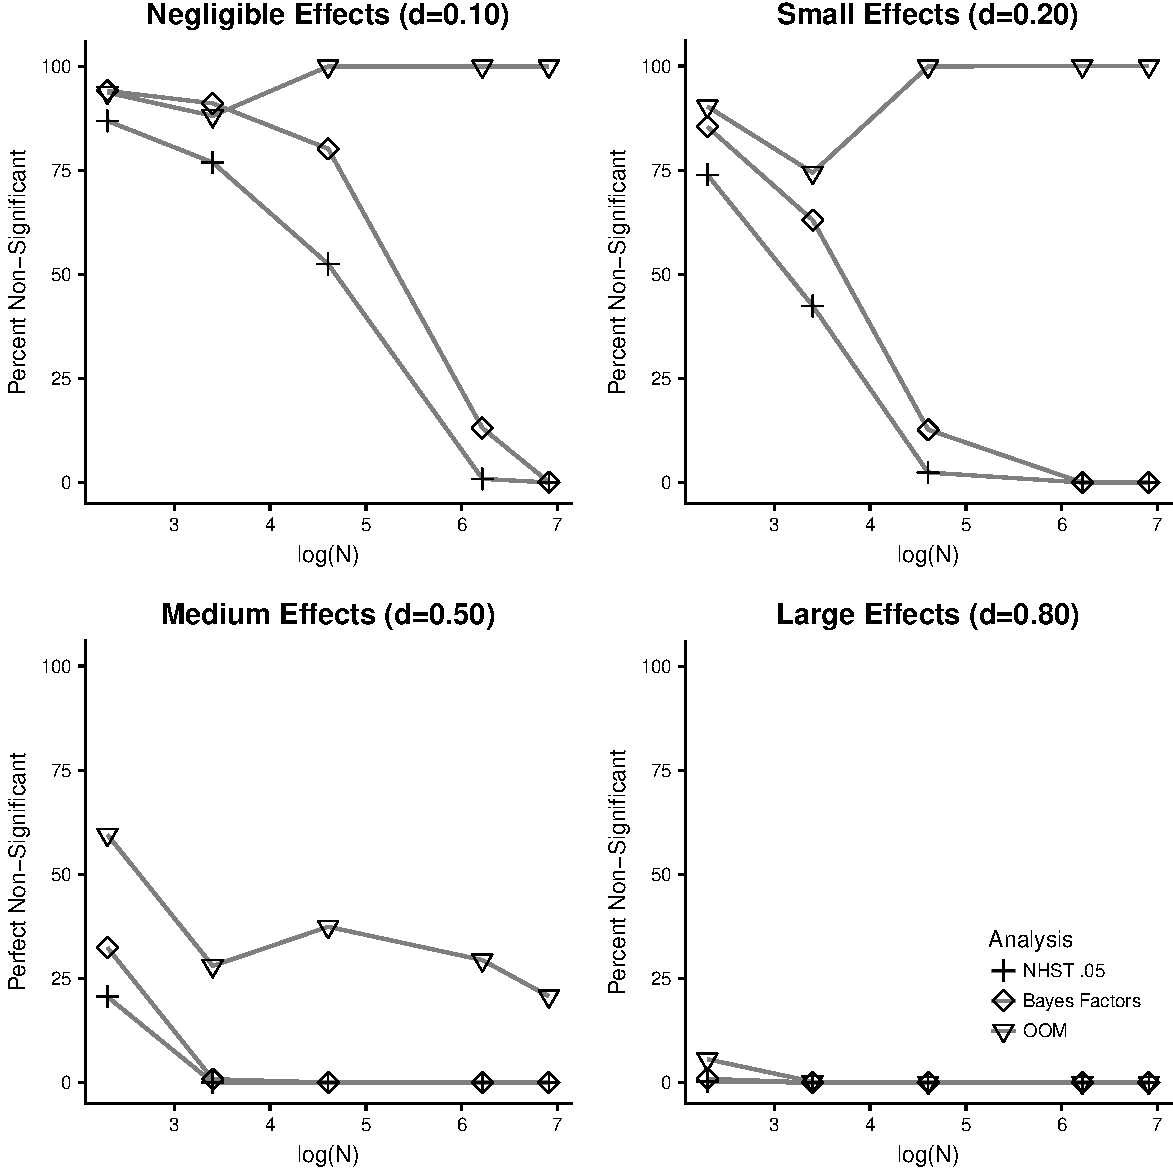
\includegraphics{alt_nhst_FINAL_files/figure-latex/effects-graph-nonsig-1.pdf}
\caption{\label{fig:effects-graph-nonsig}Percent of non-significant effects
for each analysis given effect size and sample size.}
\end{figure}

\begin{figure}
\centering
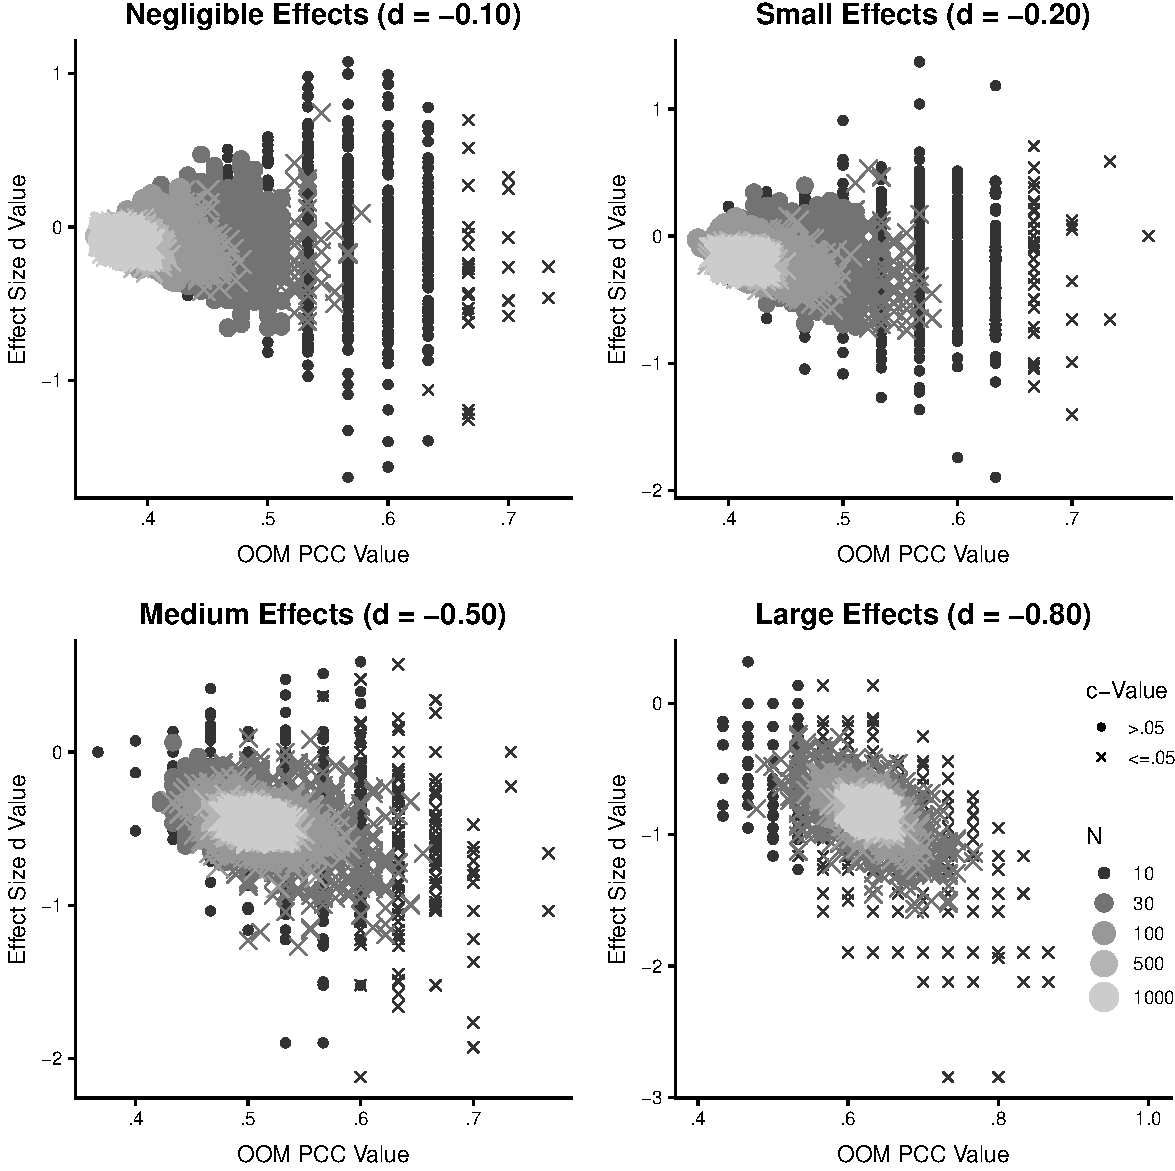
\includegraphics{alt_nhst_FINAL_files/figure-latex/effects-pcc-d-1.pdf}
\caption{\label{fig:effects-pcc-d}PCC and c-values plotted against observed
effect size (\emph{d}-values) given effect size and sample size
conditions. Xs indicate simulations with c-values \textless{} .05,which
were binned as significant if they were found in conjunction with PCC
values over .50. Point size and color indicates sample size wherein
larger samples are lighter colors. Please note that the key for the
entire set of graphics is in the bottom right hand corner.}
\end{figure}

\hypertarget{percent-agreement}{%
\subsection{Percent Agreement}\label{percent-agreement}}

A goal of this project was to expand the toolbox of options for
researchers to determine what evidence supports their hypotheses by
examining multiple methodologies. We calculated the percent of time that
all analyses agreed across overall and \emph{post hoc} comparison
estimates. Figure \ref{fig:agree-graph-omnibus} illustrates the pattern
of 100\% agreement on effects for critical omnibus tests only at each
sample size and effect size. Figure \ref{fig:agree-graph-post} portrays
the results for \emph{post hoc} tests, which only uses NHST and Bayes
Factor analyses, as OOM does not have a \emph{post hoc} test (i.e., the
test is a pattern analysis that presupposes the expected direction of
\emph{post hoc} tests).

When effect sizes were negligible and for small effects, agreement was
best across small samples and decreased across sample size, as NHST was
overly biased to report significant estimates and OOM and BF were less
likely to do so. For medium and large effect sizes, 50-75\% agreement
was found, usually regardless of sample size. Additionally, we found
that for negligible, small, and medium effects, agreement for \emph{post
hoc} tests was higher than agreement for overall comparisons. The
\emph{post hoc} comparisons for levels 1 to 2 and levels 2 to 3 were
less likely to be binned as significant across negligible and small
effects, so the agreement levels were higher for these individual
comparisons due to non-significant follow up tests. The critical omnibus
test was more likely to be significant due to the inclusion of effect of
comparisons between level 1 and 3, which were double the effect size.
However, these \emph{post hoc} comparisons do not include the
conservative significant binning from OOM, which decreased critical
omnibus 100\% agreement seen in Figure \ref{fig:agree-graph-omnibus}.
Again, the differences between \emph{p} \textless{} .05 and \emph{p}
\textless{} .005 were minimal. Complete tables of percentages of binning
across critical omnibus and \emph{post hoc} tests, along with agreement
percentages broken down by bins can be found at
\url{https://osf.io/u9hf4/?view_only=1caa9092868b4d7aadb9a83a31a979cd}.

\begin{figure}
\centering
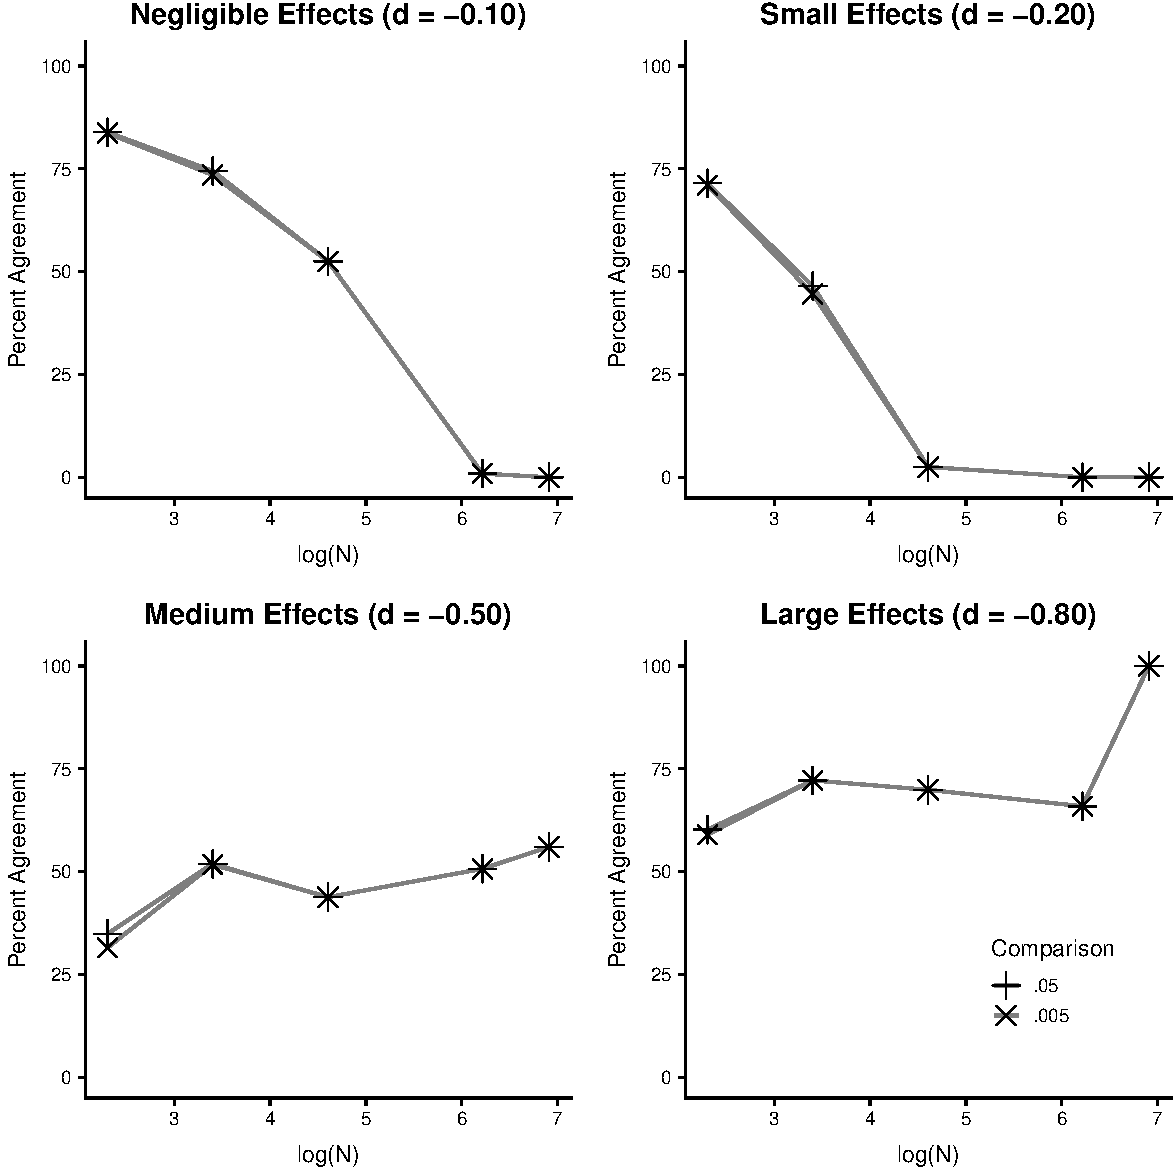
\includegraphics{alt_nhst_FINAL_files/figure-latex/agree-graph-omnibus-1.pdf}
\caption{\label{fig:agree-graph-omnibus}Percent of agreement across all
analyses given effect size and sample size for omnnibus tests.}
\end{figure}

\begin{figure}
\centering
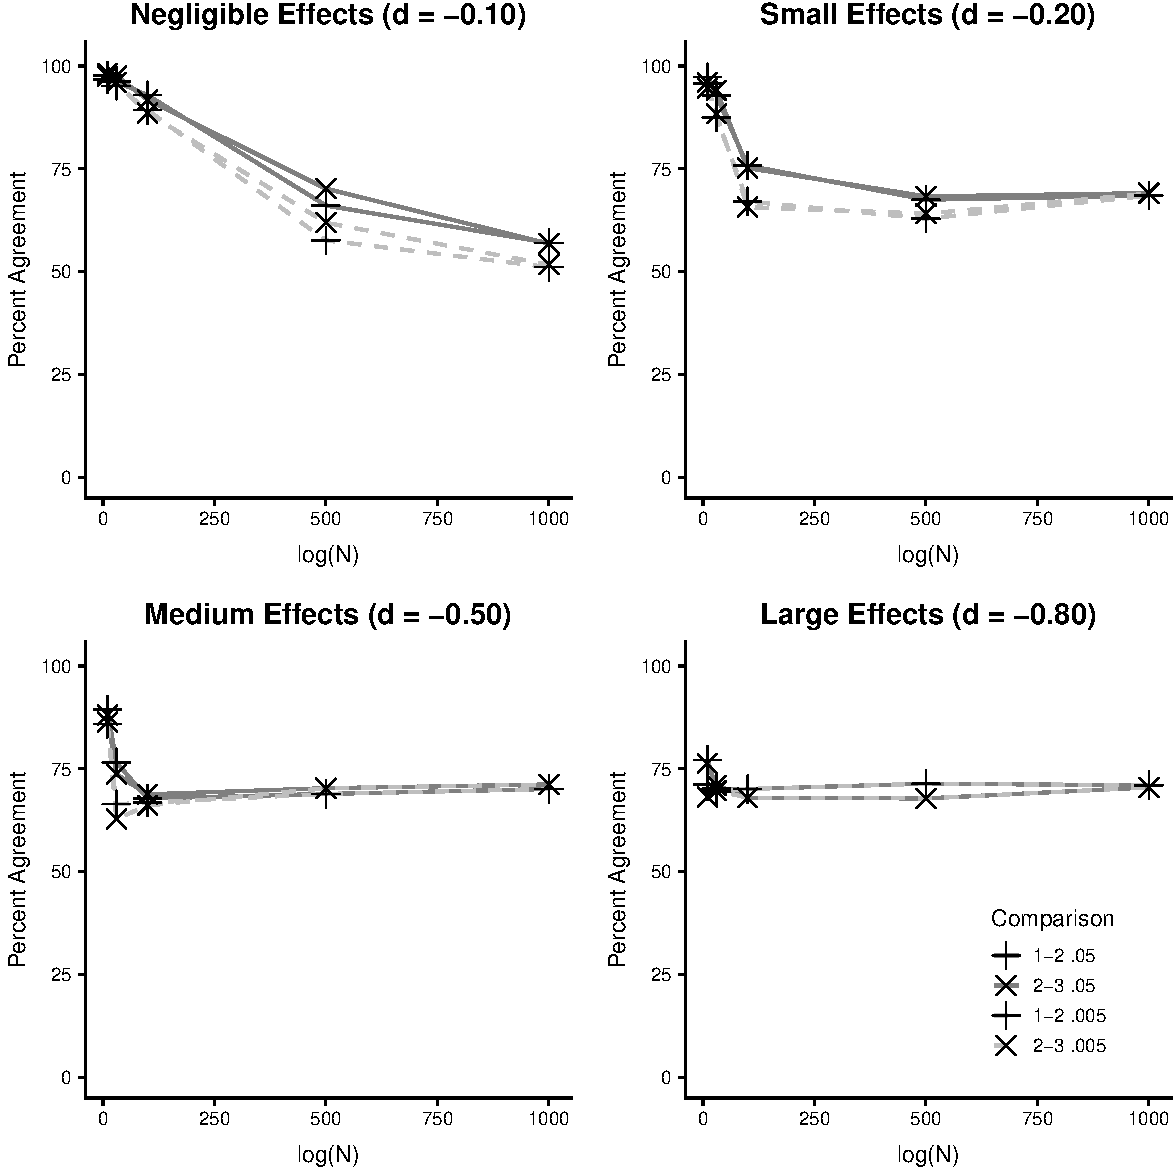
\includegraphics{alt_nhst_FINAL_files/figure-latex/agree-graph-post-1.pdf}
\caption{\label{fig:agree-graph-post}Percent of agreement across each
analysis given effect size and sample size \(post hoc\) tests with \(p\)
\textless{} .05 (solid) and \(p\) \textless{} .005 (dashed). Note that
this graph only compares the NHST and BF conclusions.}
\end{figure}

\hypertarget{criterion-comparison}{%
\subsection{Criterion Comparison}\label{criterion-comparison}}

As the relationship between BF and \emph{p}-values is already well
documented, we will not discuss them here beyond stating that we found
the expected pattern shown in previous work (Rouder et al., 2012), and
that individuals who wish to view this comparison, as well as all the
other comparisons discussed here should visit our interactive Shiny
application at our OSF page. Of interest was the comparison of OOM
indices to traditional NHST and Bayesian indices. First, in Figure
\ref{fig:pcc-bf-fig}, PCC values are plotted against log BF values and
\(p\)-values. The log of BF was taken to include all values on a
viewable axis, and all infinity values were windsorized to the next
highest point. Increasing sample size is shown by increasing point size
and lighter colors. Additionally, since OOM values are a combination of
PCC and \(c\)-values, \(c\)-values below .05 are shown as Xs instead of
dots. Therefore, all values PCC \textgreater{}= .50 that are also
denoted as Xs would be considered significant in this example. The
provided Shiny application uses color to distinguish sample size
differences, as well as includes options to create each combination
effect size and criterion individually. Only two graphs are provided
here to save space.

\begin{figure}
\centering
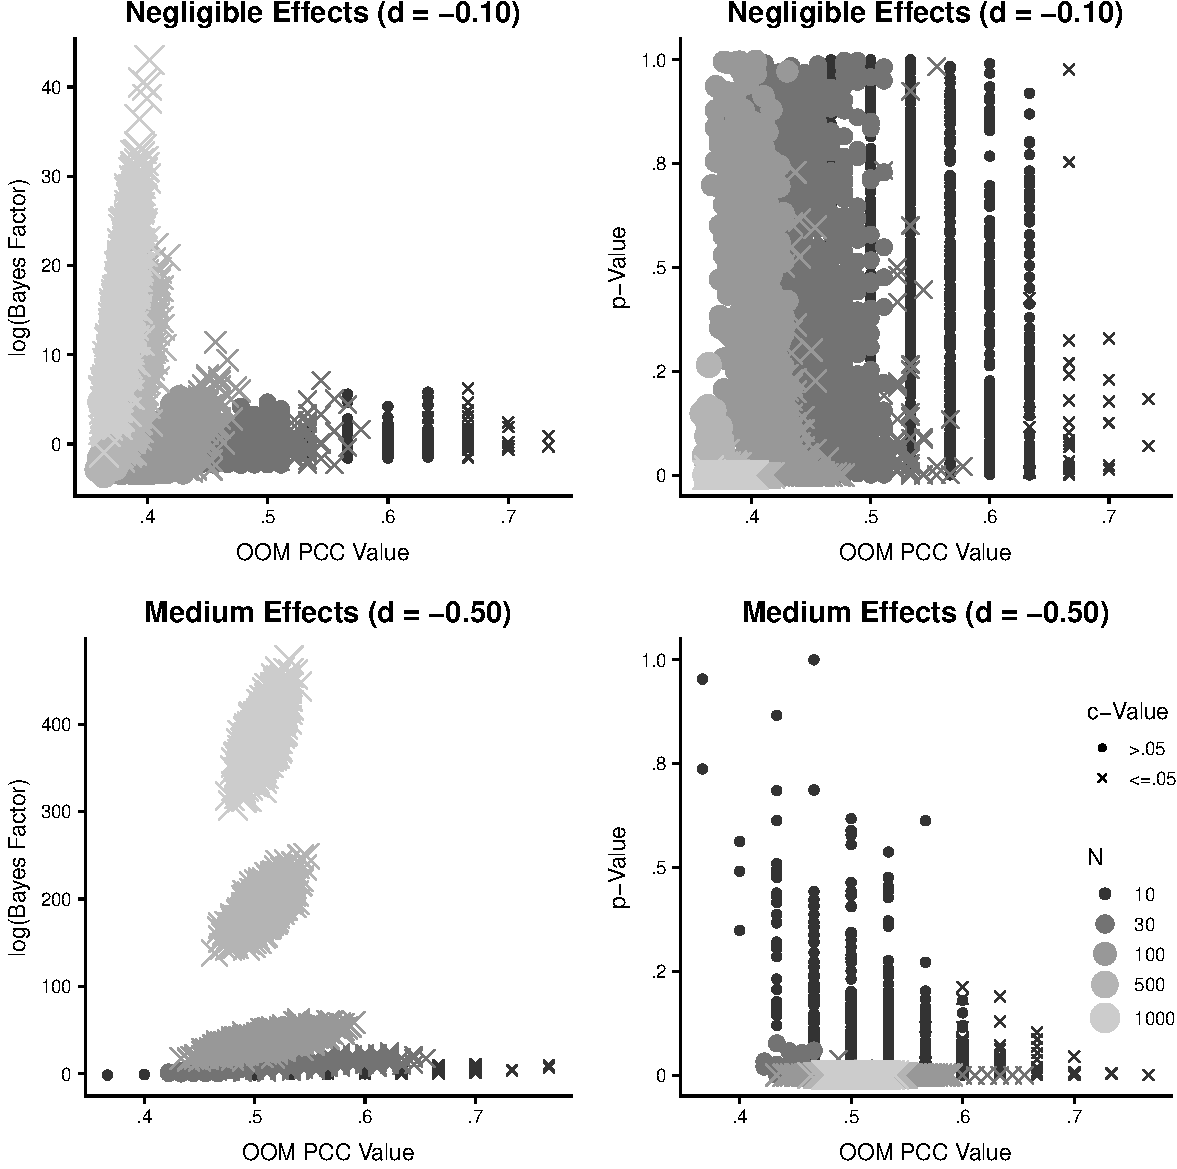
\includegraphics{alt_nhst_FINAL_files/figure-latex/pcc-bf-fig-1.pdf}
\caption{\label{fig:pcc-bf-fig}PCC and c-values plotted against \(p\) and BF
values for negligible and medium effect size conditions. Xs indicate
simulations with \(c\)-values \textless{} .05,which were binned as
significant if they were found in conjunction with PCC values over .50.
Point size and color indicates sample size wherein larger samples are
lighter colors. Please note that the key for the entire set of graphics
is in the bottom right hand corner.}
\end{figure}

In Figure \ref{fig:pcc-bf-fig}, the left hand column portrays the
relationship between log BF values and PCC values in negligible and
medium effect sizes. With negligible effect sizes, we found large
variability in PCC values across a small span of BF values while sample
sizes remained low, but as \emph{N} increased, we saw that the range of
PCC values narrowed considerably with increasing BF values. Therefore,
as sample size increased, the PCC values constricted, while BF values
expanded. A similar pattern appeared when viewing the medium sample size
graph, as again PCC values became less variable with increased sample
size, and BF tended to increase both in variability and in value as the
sample size grew. Here, we can see a benefit of PCC, along with
\(c\)-values, as increasing sample size portrayed more precision in PCC,
instead of the increased variability found in BF.

It is also important to note that within the negligible effects graph,
while many of these PCC values reached high values, that these values
did not denote patterns that would necessarily be seen as unique.
\(c\)-values were a secondary measure of evaluation that eliminated a
number of these matches from being considered meaningful. A large
majority of points with larger sample sizes on the figure included low
chance values, however, the PCC values for these simulations were lower
than a meaningful percent used for cutoff criterion. This two-step
process helped to weed out effects that were negligible, especially at
larger sample sizes.

Additionally, we compared \(p\)-values and PCC values, which are
illustrated on the right hand side of Figure \ref{fig:pcc-bf-fig}.
Again, PCC values showed far more variability with small sample sizes,
and the \(p\)-values associated with these smaller sample sizes were
also quite variable. Importantly, even when an effect was negligible,
PCC values become less variable with increasing sample size. PCC values
also indicated that there was little evidence of the hypothesized
pattern by shifting toward zero. \(p\)-values decreased in variability
at high sample sizes and shifted toward minuscule values, thus, pointing
toward rejecting the null hypothesis. With medium effect sizes, both
\(p\)-values and PCC values were variable at small sample sizes. At
larger sample sizes, \(p\)-values decreased towards floor effects (i.e.,
closer to zero), while PCC values simply narrowed in range shifting
slight above .50. The benefit of multiple criteria evaluation here was
clear, as \(p\)-values increasingly indicated significance as sample
size increased, PCC values were not effected in this way and thus
presented a more stable picture of the presence of an effect. While
multiple criteria may not completely reduce the interpretation of false
positives in the literature, the relationship between these values
illustrated that multiple indices can provided a clearer picture of the
evidentiary value available in a study.

\hypertarget{limitations}{%
\subsection{Limitations}\label{limitations}}

Within any study a number of limitations exist. The largest limitation
of our study is that we chose to focus on a simple three level repeated
measures ANOVA design. The benefit to this focus is the simplicity of
understanding the relationship between analyses, while also using a well
understood NHST procedure. However, is possible that these same
relationships may or may not exist in alternative design contexts.
Additionally, our choices for classification of significant effects for
\emph{p}-values, BF, PCC, and \emph{c}-values was based on what we
believe a reasonable researcher may designate; however, these
classifications may vary in the real world. We provide open access to
our simulations and code so that an interested party can tinker with
these choices. We believe the global conclusions would likely be similar
across changes, however, the specific percentages and patterns would
likely differ. Finally, due to the specification of our simulation we
did not violate any statistical assumptions. It is possible that the
violation of these assumptions may cause changes in the relationships we
see here.

\hypertarget{discussion}{%
\section{Discussion}\label{discussion}}

This manuscript was designed to showcase two alternative paradigms to
NHST researchers and to compare the conclusions these alternative
methodologies might make in a given data environment to those NHST would
make. We believe that the awareness of multiple methodologies might
assist in strengthening our conclusions and improving reproducibility by
giving researchers the ability to identify an optimal method given the
question at hand. Further, we believe that should a researcher utilize
multiple methodologies (e.g., analyzing and reporting both a NHST
\emph{p}-value as well as an OOM PCC value) that these estimates in
tandem can help readers to weight these various forms of evidence and
arrive at a more robust conclusion. We found that changing the threshold
at which \emph{p}-values are deemed significant had little to no effect
on conclusions, especially at large sample sizes, regardless of effect
size. This finding is notable as the article by Benjamin et al. (2018)
states that an increase in sample size is likely to decrease false
positives \enquote{by factors greater than two} (p.~10), and work by
Pericchi and Pereira (2016) state that an adaptive level of significance
would be beneficial in these circumstances---neither of which are not
supported by our simulations. Our science will not grow by moving the
significance line in the sand, as this line has already been shown to
have \enquote{no ontological basis} (Rosnow \& Rosenthal, 1989, p.
1277).

Instead, we need to embrace the multitude of perspectives available to
us and to begin to employ these diverse approaches. While NHST can still
serve us well when properly utilized, it is important for researchers to
understand that different methods seek to answer different questions,
and that we need to ensure that we are using the right method to answer
a given question. When evaluating evidence in order to answer these
questions we must be wary of looking for significant differences and
focus instead on finding meaningful differences. By combining these
approaches we may be better able to qualify the strength of our evidence
and discuss a more nuanced version of our data. Additionally, while all
of these methods have drawbacks, when used in combination these methods
can begin to overcome many of these limitations. For instance, given a
large sample size, we would expect BF values to be very large and
\emph{p}-values to be very small, both indicating that the null
model/hypothesis should not be supported. However, if we also have a PCC
value of .30, we may decide that it is possible that this effect is very
small and possibly negligible. This multifaceted approach can help to
curb our enthusiasm over small or negligible \enquote{significant}
effects that may not be practically meaningful and possibly may not
replicate. Regardless if analyses agree or disagree on the presence of
an effect, a researcher can investigate the direction and size of the
effect, the proportion of data that agrees or disagrees with the
direction of the effect, and discuss conclusions accordingly. Each
methodology behaves slightly differently in given data environments,
which might begin to highlight meaningful differences when discussed
together.

Some may contest that all of these analyses are capable of being hacked,
like \emph{p}-values, through researcher degrees of freedom, choice of
priors, or pattern choice, among other actions (Simmons et al., 2011).
Transparency throughout the research process is key to eliminating these
issues, as \(\alpha\) changes may only encourage bad research practices
with the current incentive structure on publishing. Although we have the
capability to share research across the world, research often still
occurs behind closed doors. The Open Science Framework grants insight
into research processes, allowing researchers to share their
methodologies, code, design, and other important components of their
projects. In addition to posting materials for projects,
pre-registration of hypotheses and methodology will be an important
facet in scientific accountability. Further, with increased transparency
editors and other researchers can weigh the evidence presented according
to their own beliefs.

Our key suggestion in this project is the redefinition of evidentiary
value. The current focus on \emph{p}-values has shown to be problematic,
as many of the studies from the Open Science Collaboration (2015) do not
replicate at \emph{p}\textless{} .05 or \emph{p} \textless{} .005
(Lakens et al., 2018). With the change in transparency mentioned above,
publishing research with solid research designs and statistics,
regardless of \emph{p}-values, will allow for a broader range of
evidence to become available. Publishing null findings is critical in
replication and extension for discovering the limits and settings
necessary for phenomena. Registered replications and reports will allow
studies to be accepted prior to results being known, thus allowing
researchers to focus on experimental design and hypotheses
\emph{apriori} instead of \emph{p}-values \emph{post hoc}. Reports
should describe multiple indicators of evidence, such as effect sizes,
confidence intervals, power analyses, Bayes Factors, and other
descriptive statistics (Finkel, Eastwick, \& Reis, 2015; Nosek \&
Lakens, 2014; van't Veer \& Giner-Sorolla, 2016).

A misunderstanding of statistical power still plagues psychological
sciences (Bakker, Hartgerink, Wicherts, \& van der Maas, 2016), and the
effect of sample size, especially small ones, was shown here by
comparing the criterion available in these analyses. Often, individual
research labs may not have the means to adequately power a proposed
study. Multilab studies and collaboration with other scientists is
fundamental to alleviating these issues, while encouraging
interdisciplinary science. Collaboration increases our statistical
abilities, as every researcher cannot be expected to be proficient in
all methods and analyses, but teams of researchers can be assembled to
cover a wider range of statistical skills to provide adequate estimates
of evidence in their reports. We understand that there may be resistance
to the implementation of multiple methodologies as these new
methodologies take time and effort to learn. However, through the use of
free programs (JASP, R, OOM, Shiny) and tutorials (YouTube, Coursera,
\url{http://www.statstools.com}), we believe all researchers are capable
of learning these analyses. We believe that through the expansion of our
analytical knowledge and application of these new methodologies, we can
begin to attenuate some of the strain currently placed on psychological
science and to increase the strength of evidence in our discipline.

\newpage

\hypertarget{references}{%
\section{References}\label{references}}

\setlength{\parindent}{-0.5in}
\setlength{\leftskip}{0.5in}

\hypertarget{refs}{}
\leavevmode\hypertarget{ref-AmericanPsychologicalAssociation2010}{}%
American Psychological Association. (2010). \emph{Publication manual of
the American Psychological Association} (6th ed.). American
Psychological Association.

\leavevmode\hypertarget{ref-Aust2017}{}%
Aust, F., \& Barth, M. (2017). papaja: Create APA manuscripts with R
Markdown. Retrieved from \url{https://github.com/crsh/papaja}

\leavevmode\hypertarget{ref-Bakker2016}{}%
Bakker, M., Hartgerink, C. H. J., Wicherts, J. M., \& van der Maas, H.
L. J. (2016). Researchers' intuitions about power in psychological
research. \emph{Psychological Science}, \emph{27}(8), 1069--1077.
doi:\href{https://doi.org/10.1177/0956797616647519}{10.1177/0956797616647519}

\leavevmode\hypertarget{ref-Bakker2012}{}%
Bakker, M., van Dijk, A., \& Wicherts, J. M. (2012). The rules of the
game called psychological science. \emph{Perspectives on Psychological
Science}, \emph{7}(6), 543--554.
doi:\href{https://doi.org/10.1177/1745691612459060}{10.1177/1745691612459060}

\leavevmode\hypertarget{ref-Bellhouse2004}{}%
Bellhouse, D. R. (2004). The Reverend Thomas Bayes, FRS: A Biography to
celebrate the tercentenary of his birth. \emph{Statistical Science},
\emph{19}(1), 3--43.
doi:\href{https://doi.org/10.1214/088342304000000189}{10.1214/088342304000000189}

\leavevmode\hypertarget{ref-Benjamin2017}{}%
Benjamin, D. J., Berger, J. O., Johannesson, M., Nosek, B. A.,
Wagenmakers, E.-J., Berk, R., \ldots{} Johnson, V. E. (2018). Redefine
statistical significance. \emph{Nature Human Behaviour}, \emph{2}(1),
6--10.
doi:\href{https://doi.org/10.1038/s41562-017-0189-z}{10.1038/s41562-017-0189-z}

\leavevmode\hypertarget{ref-Buchanan2017}{}%
Buchanan, E. M., Valentine, K. D., \& Scofield, J. E. (2017). MOTE.
Retrieved from \url{https://github.com/doomlab/MOTE}

\leavevmode\hypertarget{ref-Cohen1992a}{}%
Cohen, J. (1992). A power primer. \emph{Psychological Bulletin},
\emph{112}(1), 155--159.
doi:\href{https://doi.org/10.1037/0033-2909.112.1.155}{10.1037/0033-2909.112.1.155}

\leavevmode\hypertarget{ref-Cumming2008}{}%
Cumming, G. (2008). Replication and p intervals. \emph{Perspectives on
Psychological Science}, \emph{3}(4), 286--300.
doi:\href{https://doi.org/10.1111/j.1745-6924.2008.00079.x}{10.1111/j.1745-6924.2008.00079.x}

\leavevmode\hypertarget{ref-Cumming2014}{}%
Cumming, G. (2014). The new statistics: Why and how. \emph{Psychological
Science}, \emph{25}(1), 7--29.
doi:\href{https://doi.org/10.1177/0956797613504966}{10.1177/0956797613504966}

\leavevmode\hypertarget{ref-Datta1996}{}%
Datta, G., \& Ghosh, M. (1996). On the invariance of noninformative
priors. \emph{The Annals of Statistics}, \emph{24}(1), 141--159.
doi:\href{https://doi.org/10.1214/aos/1033066203}{10.1214/aos/1033066203}

\leavevmode\hypertarget{ref-DeLaplace1774}{}%
De Laplace, P. S. (1774). Mémoire sur les suites récurro-récurrentes et
sur leurs usages dans la théorie des hasards. \emph{Mém. Acad. R. Sci.
Paris}, \emph{6}(8), 353--371. Retrieved from
\href{http://cerebro.cs.xu.edu/math/Sources/Laplace/recurro\%7B/_\%7Drecurrentes.pdf}{http://cerebro.cs.xu.edu/math/Sources/Laplace/recurro\{\textbackslash{}\_\}recurrentes.pdf}

\leavevmode\hypertarget{ref-Dienes2008}{}%
Dienes, Z. (2008). \emph{Understanding psychology as a science: an
introduction to scientific and statistical inference}. Palgrave
Macmillan.

\leavevmode\hypertarget{ref-Dienes2014}{}%
Dienes, Z. (2014). Using Bayes to get the most out of non-significant
results. \emph{Frontiers in Psychology}, \emph{5}(July), 1--17.
doi:\href{https://doi.org/10.3389/fpsyg.2014.00781}{10.3389/fpsyg.2014.00781}

\leavevmode\hypertarget{ref-Etz2016}{}%
Etz, A., \& Vandekerckhove, J. (2016). A Bayesian perspective on the
reproducibility project: Psychology. \emph{PLoS ONE}, \emph{11}(2),
1--12.
doi:\href{https://doi.org/10.1371/journal.pone.0149794}{10.1371/journal.pone.0149794}

\leavevmode\hypertarget{ref-Finkel2015}{}%
Finkel, E. J., Eastwick, P. W., \& Reis, H. T. (2015). Best research
practices in psychology: Illustrating epistemological and pragmatic
considerations with the case of relationship science. \emph{Journal of
Personality and Social Psychology}, \emph{108}(2), 275--297.
doi:\href{https://doi.org/10.1037/pspi0000007}{10.1037/pspi0000007}

\leavevmode\hypertarget{ref-Fisher1932}{}%
Fisher, R. A. (1932). Inverse probability and the use of Likelihood.
\emph{Mathematical Proceedings of the Cambridge Philosophical Society},
\emph{28}(3), 257--261.
doi:\href{https://doi.org/10.1017/S0305004100010094}{10.1017/S0305004100010094}

\leavevmode\hypertarget{ref-Gelman2004}{}%
Gelman, A., Carlin, J. B., Stern, H. S., \& Rubin, D. R. (2013).
\emph{Bayesian data analysis}. Chapman \& Hall/CRC.

\leavevmode\hypertarget{ref-Genz2017}{}%
Genz, A., Bretz, F., Miwa, T., Mi, X., Leisch, F., Scheipl, F., \&
Hothorn, T. (2017). mvtnorm: Multivariate normal and t distributions.
Retrieved from \url{http://cran.r-project.org/package=mvtnorm}

\leavevmode\hypertarget{ref-Gigerenzer2004}{}%
Gigerenzer, G. (2004). Mindless statistics. \emph{The Journal of
Socio-Economics}, \emph{33}(5), 587--606.
doi:\href{https://doi.org/10.1016/j.socec.2004.09.033}{10.1016/j.socec.2004.09.033}

\leavevmode\hypertarget{ref-Gigerenzer2004a}{}%
Gigerenzer, G., Krauss, S., \& Vitouch, O. (2004). The null ritual: What
you always wanted to know about significance testing but were afraid to
ask. In \emph{The sage handbook of quantitative methodology for the
social sciences} (pp. 392--409). Thousand Oaks, CA: SAGE Publications,
Inc.
doi:\href{https://doi.org/10.4135/9781412986311.n21}{10.4135/9781412986311.n21}

\leavevmode\hypertarget{ref-Grice2011}{}%
Grice, J. W. (2011). \emph{Observation Oriented Modeling: Analysis of
cause in the behavioral sciences} (p. 242). Elsevier/Academic Press.

\leavevmode\hypertarget{ref-Grice2014}{}%
Grice, J. W. (2014). Observation Oriented Modeling: Preparing students
for research in the 21st century. \emph{Comprehensive Psychology},
\emph{3}, 05.08.IT.3.3.
doi:\href{https://doi.org/10.2466/05.08.IT.3.3}{10.2466/05.08.IT.3.3}

\leavevmode\hypertarget{ref-Grice2012}{}%
Grice, J. W., Barrett, P. T., Schlimgen, L. A., \& Abramson, C. I.
(2012). Toward a brighter future for psychology as an observation
oriented science. \emph{Behavioral Sciences}, \emph{2}(4), 1--22.
doi:\href{https://doi.org/10.3390/bs2010001}{10.3390/bs2010001}

\leavevmode\hypertarget{ref-Grice2015}{}%
Grice, J. W., Craig, D. P. A., \& Abramson, C. I. (2015). A simple and
transparent alternative to repeated measures ANOVA. \emph{SAGE Open},
\emph{5}(3), 2158244015604192.
doi:\href{https://doi.org/10.1177/2158244015604192}{10.1177/2158244015604192}

\leavevmode\hypertarget{ref-Haaf2017}{}%
Haaf, J., \& Rouder, J. N. (2017). \emph{Developing constraint in
bayesian mixed models}.
doi:\href{https://doi.org/10.17605/OSF.IO/KTJNQ}{10.17605/OSF.IO/KTJNQ}

\leavevmode\hypertarget{ref-Ioannidis2005}{}%
Ioannidis, J. P. A. (2005). Why most published research findings are
false. \emph{PLoS Medicine}, \emph{2}(8), e124.
doi:\href{https://doi.org/10.1371/journal.pmed.0020124}{10.1371/journal.pmed.0020124}

\leavevmode\hypertarget{ref-JASPTeam2017}{}%
JASP Team. (2017). JASP. Retrieved from \url{https://jasp-stats.org/}

\leavevmode\hypertarget{ref-Kass1995a}{}%
Kass, R. E., \& Raftery, A. E. (1995). Bayes Factors. \emph{Journal of
the American Statistical Association}, \emph{90}(430), 773--795.
doi:\href{https://doi.org/10.2307/2291091}{10.2307/2291091}

\leavevmode\hypertarget{ref-Klugkist2007}{}%
Klugkist, I., \& Hoijtink, H. (2007). The Bayes factor for inequality
and about equality constrained models. \emph{Computational Statistics \&
Data Analysis}, \emph{51}(12), 6367--6379.
doi:\href{https://doi.org/10.1016/j.csda.2007.01.024}{10.1016/j.csda.2007.01.024}

\leavevmode\hypertarget{ref-Kruschke2014}{}%
Kruschke, J. K. (2014). \emph{Doing Bayesian data analysis: A tutorial
with R, JAGS, and Stan} (2nd ed.). Academic Press.

\leavevmode\hypertarget{ref-Lakens2013}{}%
Lakens, D. (2013). Calculating and reporting effect sizes to facilitate
cumulative science: A practical primer for t-tests and ANOVAs.
\emph{Frontiers in Psychology}, \emph{4}.
doi:\href{https://doi.org/10.3389/fpsyg.2013.00863}{10.3389/fpsyg.2013.00863}

\leavevmode\hypertarget{ref-Lakens2017a}{}%
Lakens, D. (2017). Equivalence tests. \emph{Social Psychological and
Personality Science}, \emph{8}(4), 355--362.
doi:\href{https://doi.org/10.1177/1948550617697177}{10.1177/1948550617697177}

\leavevmode\hypertarget{ref-Lakens2017}{}%
Lakens, D., Adolfi, F. G., Albers, C. J., Anvari, F., Apps, M. A. J.,
Argamon, S. E., \ldots{} Zwaan, R. A. (2018). Justify your alpha.
\emph{Nature Human Behaviour}, \emph{2}(3), 168--171.
doi:\href{https://doi.org/10.1038/s41562-018-0311-x}{10.1038/s41562-018-0311-x}

\leavevmode\hypertarget{ref-Lawrence2017}{}%
Lawrence, M. A. (2017). ez: Easy analysis and visualization of factorial
experiments. Retrieved from \url{http://cran.r-project.org/package=ez}

\leavevmode\hypertarget{ref-Lehmann1993}{}%
Lehmann, E. L. (1993). The Fisher, Neyman-Pearson theories of testing
hypotheses: One theory or two? \emph{Journal of the American Statistical
Association}, \emph{88}(424), 1242--1249.
doi:\href{https://doi.org/10.1080/01621459.1993.10476404}{10.1080/01621459.1993.10476404}

\leavevmode\hypertarget{ref-Lehmann2011}{}%
Lehmann, E. L. (2011). \emph{Fisher, Neyman, and the creation of
classical statistics}. New York, NY: Springer.

\leavevmode\hypertarget{ref-Lindsay2015}{}%
Lindsay, D. S. (2015). Replication in Psychological Science.
\emph{Psychological Science}, \emph{26}(12), 1827--1832.
doi:\href{https://doi.org/10.1177/0956797615616374}{10.1177/0956797615616374}

\leavevmode\hypertarget{ref-Maxwell2004}{}%
Maxwell, S. E., \& Delaney, H. D. (2004). \emph{Designing experiments
and analyzing data: A model comparison perspective} (2nd ed.). Mahwah,
NJ: Lawrence Erlbaum Associates.

\leavevmode\hypertarget{ref-Maxwell2015}{}%
Maxwell, S. E., Lau, M. Y., \& Howard, G. S. (2015). Is psychology
suffering from a replication crisis? What does ``failure to replicate''
really mean? \emph{American Psychologist}, \emph{70}(6), 487--498.
doi:\href{https://doi.org/10.1037/a0039400}{10.1037/a0039400}

\leavevmode\hypertarget{ref-Morey2015c}{}%
Morey, R. D. (2015). On verbal categories for the interpretation of
Bayes factors. Retrieved from
\url{http://bayesfactor.blogspot.com/2015/01/on-verbal-categories-for-interpretation.html}

\leavevmode\hypertarget{ref-Morey2015b}{}%
Morey, R. D., \& Rouder, J. N. (2015). BayesFactor: Computation of Bayes
Factors for common designs. Retrieved from
\url{https://cran.r-project.org/package=BayesFactor}

\leavevmode\hypertarget{ref-Nosek2014}{}%
Nosek, B. A., \& Lakens, D. (2014). Registered reports. \emph{Social
Psychology}, \emph{45}(3), 137--141.
doi:\href{https://doi.org/10.1027/1864-9335/a000192}{10.1027/1864-9335/a000192}

\leavevmode\hypertarget{ref-Nosek2012}{}%
Nosek, B. A., Spies, J. R., \& Motyl, M. (2012). Scientific utopia.
\emph{Perspectives on Psychological Science}, \emph{7}(6), 615--631.
doi:\href{https://doi.org/10.1177/1745691612459058}{10.1177/1745691612459058}

\leavevmode\hypertarget{ref-OpenScienceCollaboration2015}{}%
Open Science Collaboration. (2015). Estimating the reproducibility of
psychological science. \emph{Science}, \emph{349}(6251),
aac4716--aac4716.
doi:\href{https://doi.org/10.1126/science.aac4716}{10.1126/science.aac4716}

\leavevmode\hypertarget{ref-Pericchi2016}{}%
Pericchi, L., \& Pereira, C. (2016). Adaptative significance levels
using optimal decision rules: Balancing by weighting the error
probabilities. \emph{Brazilian Journal of Probability and Statistics},
\emph{30}(1), 70--90.
doi:\href{https://doi.org/10.1214/14-BJPS257}{10.1214/14-BJPS257}

\leavevmode\hypertarget{ref-Press2002}{}%
Press, S. J. (2002). \emph{Subjective and objective Bayesian statistics}
(2nd ed.). Hoboken, NJ, USA: John Wiley \& Sons, Inc.
doi:\href{https://doi.org/10.1002/9780470317105}{10.1002/9780470317105}

\leavevmode\hypertarget{ref-Rosnow1989}{}%
Rosnow, R. L., \& Rosenthal, R. (1989). Statistical procedures and the
justification of knowledge in psychological science. \emph{American
Psychologist}, \emph{44}(10), 1276--1284.
doi:\href{https://doi.org/10.1037/0003-066X.44.10.1276}{10.1037/0003-066X.44.10.1276}

\leavevmode\hypertarget{ref-Rouder2012}{}%
Rouder, J. N., Morey, R. D., Speckman, P. L., \& Province, J. M. (2012).
Default Bayes factors for ANOVA designs. \emph{Journal of Mathematical
Psychology}, \emph{56}(5), 356--374.
doi:\href{https://doi.org/10.1016/j.jmp.2012.08.001}{10.1016/j.jmp.2012.08.001}

\leavevmode\hypertarget{ref-Rouder2009}{}%
Rouder, J. N., Speckman, P. L., Sun, D., Morey, R. D., \& Iverson, G.
(2009). Bayesian t tests for accepting and rejecting the null
hypothesis. \emph{Psychonomic Bulletin \& Review}, \emph{16}(2),
225--237.
doi:\href{https://doi.org/10.3758/PBR.16.2.225}{10.3758/PBR.16.2.225}

\leavevmode\hypertarget{ref-Sauer2016}{}%
Sauer, S., \& Luebke, K. (2016, January). Observation Oriented Modeling
revised from a statistical point of view.
doi:\href{https://doi.org/10.17605/OSF.IO/3J4XR}{10.17605/OSF.IO/3J4XR}

\leavevmode\hypertarget{ref-Sellke2001}{}%
Sellke, T., Bayarri, M. J., \& Berger, J. O. (2001). Calibration of p
values for testing precise null hypotheses. \emph{American
Statistician}, \emph{55}(1), 62--71.
doi:\href{https://doi.org/10.1198/000313001300339950}{10.1198/000313001300339950}

\leavevmode\hypertarget{ref-Simmons2011}{}%
Simmons, J. P., Nelson, L. D., \& Simonsohn, U. (2011). False-positive
psychology: Undisclosed flexibility in data collection and analysis
allows presenting anything as significant. \emph{Psychological Science},
\emph{22}(11), 1359--1366.
doi:\href{https://doi.org/10.1177/0956797611417632}{10.1177/0956797611417632}

\leavevmode\hypertarget{ref-Tabachnick2012}{}%
Tabachnick, B. G., \& Fidell, L. S. (2012). \emph{Using multivariate
statistics} (Sixth.). Boston, MA: Pearson.

\leavevmode\hypertarget{ref-Valentine2013}{}%
Valentine, K. D., \& Buchanan, E. M. (2013). JAM-boree: An application
of observation oriented modelling to judgements of associative memory.
\emph{Journal of Cognitive Psychology}, \emph{25}(4), 400--422.
doi:\href{https://doi.org/10.1080/20445911.2013.775120}{10.1080/20445911.2013.775120}

\leavevmode\hypertarget{ref-VanElk2015}{}%
van Elk, M., Matzke, D., Gronau, Q. F., Guan, M., Vandekerckhove, J., \&
Wagenmakers, E.-J. (2015). Meta-analyses are no substitute for
registered replications: A skeptical perspective on religious priming.
\emph{Frontiers in Psychology}, \emph{6}, 1365.
doi:\href{https://doi.org/10.3389/fpsyg.2015.01365}{10.3389/fpsyg.2015.01365}

\leavevmode\hypertarget{ref-VantVeer2016}{}%
van't Veer, A. E., \& Giner-Sorolla, R. (2016). Pre-registration in
social psychology---A discussion and suggested template. \emph{Journal
of Experimental Social Psychology}, \emph{67}, 2--12.
doi:\href{https://doi.org/10.1016/j.jesp.2016.03.004}{10.1016/j.jesp.2016.03.004}

\leavevmode\hypertarget{ref-Wagenmakers2007}{}%
Wagenmakers, E.-J. (2007). A practical solution to the pervasive
problems of p values. \emph{Psychonomic Bulletin \& Review},
\emph{14}(5), 779--804.
doi:\href{https://doi.org/10.3758/BF03194105}{10.3758/BF03194105}

\leavevmode\hypertarget{ref-Wasserstein2016}{}%
Wasserstein, R. L., \& Lazar, N. A. (2016). The ASA's statement on p
-values: Context, process, and purpose. \emph{The American
Statistician}, \emph{70}(2), 129--133.
doi:\href{https://doi.org/10.1080/00031305.2016.1154108}{10.1080/00031305.2016.1154108}

\leavevmode\hypertarget{ref-Wetzels2011}{}%
Wetzels, R., Matzke, D., Lee, M. D., Rouder, J. N., Iverson, G. J., \&
Wagenmakers, E.-J. (2011). Statistical evidence in experimental
psychology. \emph{Perspectives on Psychological Science}, \emph{6}(3),
291--298.
doi:\href{https://doi.org/10.1177/1745691611406923}{10.1177/1745691611406923}


\end{document}
